%%
\label{chap-WAD}


Here some properties of the algorithm given in \secref{mdsdist} are given.

\section{Preliminaries}

To begin with some preliminaries. Notation is as in \secref{mdsdist}, but is refreshed here. In this section a proof of the uniqueness of the shortest path in a simple polygon is given.

\subsection{Notation}

Here follows a list of mathematical objects used in the next section which may be useful for reference.It may also be useful to refer back to section \ref{mdsdist}.
\begin{itemize}
   \item $p_1$ and $p_2$ always refer to the two points between which the shortest path is to be found.
   \item $\Gamma$ is the polygon that the shortest path is to be found with respect to. $\Gamma$ is a simple polygon, meaning that it contains no holes.
   \item $v_i$ refers to a point in a path within the domain, it may or may not be a vertex of $\Gamma$.
   \item $\mathcal{P}_1$ and $\mathcal{P}_2$ are the initial paths between $p_1$ and $p_2$ that trace the boundary.
   \item $\mathcal{P}$ is the working path between $p_1$ and $p_2$.
   \item$\mathcal{S}_{i}$ is a section of a path.
\end{itemize}

\subsection{Terminology}

The word triangle here is used to refer to the case in which three points, $(v_i,v_{i+1},v_{i+2})$ (in $\mathcal{P}$ are vertices of a triangle all the edges of which do not cross the boundary of $\Gamma$. These are the cases in which the DELETE would simplify $(v_i,v_{i+1},v_{i+2})$ to $(v_i,v_{i+2})$.


\subsection{Uniqueness of shortest path}
\label{app-unique-sp}
Propostition: there is one, unique shortest path between point $p_1$ and $p_2$ within a simple polygon, $\Gamma$.

Proof: This is simple to see since if the shortest path were non-unique then there would exist $\mathcal{P}_A$ and  $\mathcal{P}_B$ which were both shortest paths between $p_1$ and $p_2$. It would then be the case there there would be two points $v_1^*$ and $v_2^*$ say where the paths started to differ and ended differing (these could be $p_1$ and $p_2$): the points at which $\mathcal{P}_A$ and  $\mathcal{P}_B$ become disjoint. Call the two paths that lie between $v_1^*$ and $v_2^*$ $\mathcal{S}_{AB}$ and $\mathcal{S}_{BA}$. 

Joining up $\mathcal{S}_{AB}$ and $\mathcal{S}_{BA}$ at $v_1^*$ and $v_2^*$ forms a loop, $\mathcal{L}$, say. There is nothing in the middle of $\mathcal{L}$ (since $\Gamma$ has no holes), in which case there must be a kink in at least one of the paths (since they are not identical, at least one of them must not be a straight line between $v_1^*$ and $v_2^*$), this means that there is a triangle in (at least) one of the paths, which can be straightened ($\mathcal{L}$ does not contain any obstacle stopping this) so the path is not a shortest path and can be shortened. This is a contradiction, therefore the shortest path must be unique. Figure \ref{app-WAD-unique-dia} may be helpful.

This proof was adapted from the one given in lecture notes by Leonidas Guibas available at \url{http://graphics.stanford.edu/courses/cs268-09-winter/}.


\begin{figure}
\centering
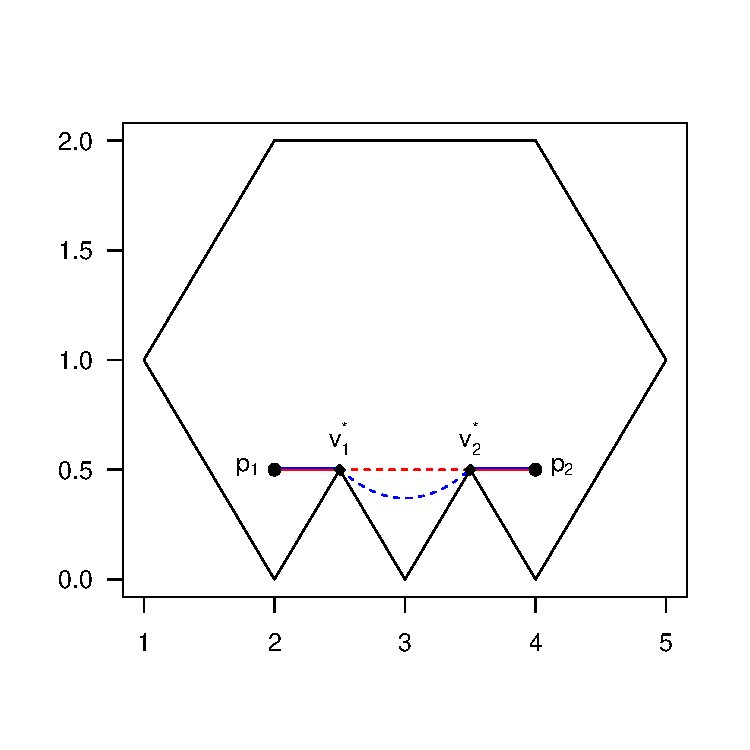
\includegraphics[width=3in]{app-WAD/figs/unique-path-dia.pdf} \\
\caption{Illustration of some of the terms used in the proof that there is always a unique shortest path. $\mathcal{P}_A$ and  $\mathcal{P}_B$ are given by the red and blue lines. The loop ($\mathcal{L}$) is given by the dotted lines; the red part is  $\mathcal{S}_{AB}$ and the blue part  $\mathcal{S}_{BA}$.}
\label{app-WAD-unique-dia}
% generated by thesis/app-WAD/figs/unique-shortest-path.R
\end{figure}

\section{Properties}

%\subsection{The algorithm terminates}
%
%The condition to be fulfilled for the algorithm to terminate is that in two consecutive runs the path does not change.
%
%First note that the ALTER step can act as (a less efficient) DELETE step: $\mathcal{P}_{I}$ would be the triplet $(v_i,v_{i+1},v_{i+2})$ (a triangle) then the DELETE substep removes $v_{i+1}$, giving $(v_i,v_{i+2})$), which would then be $\mathcal{P}_{ID}$ which could be inserted into the path. For this reason we only need to consider the ALTER step here.
%
%For the path not to change we just require that both DELETE and ALTER steps do not change the path. In the best case this happens when the path is the shortest, since there are no modifications we can make to obtain a shorter path (since the path is unique, once it has been reached, there are no other possible modifications that can be made).
%
%In the worst case one might imagine that the algorithm could get caught in a loop. This cannot happen since this would require that the ALTER step proposed shorter paths at every iteration (since otherwise they would not be accepted) \textit{ad infinitum}. This would imply that at every stage a shorter path were possible (since only shorter, not equal length modifications are accepted), clearly this cannot be the case.
%
\subsection{The algorithm terminates at the shortest path}

By definition it is clear that the algorithm must terminate at the point at which no further DELETE or ALTER steps will shorten the path. However, what is not clear is that it will terminate at the shortest path within the domain.

Say we have a locally optimal path, $P_l$. This path is locally optimal in the sense that any small perturbation of the points in $P_l$ does not yield a shorter path (i.e. the algorithm has converged) but the vertices of $P_l$ are not all identical to those of the unique (globally) shortest path $P_o$. The following argument shows that $P_l$ cannot exist. 

As in the above proof of the uniqueness of the shortest path, consider the loop $L$, formed by taking the first and last disjoint vertices of $P_l$ and $P_o$ and those points between, those points in $L$ belonging to $P_o$ are denoted $L_o$ and similarly those points belonging to $P_l$ are denoted $L_l$ (i.e. intersection of $L_l$ and $L_o$ are the start and ends of the disjointness). It must always be possible to move the points in $L_l$ towards $L_o$ smoothly (i.e. continuously through space) since there are no holes in the domain. This deformation must always continuously reduce the overall path length of $P_l$.

Now it remains to be shown that such a deformation can be performed by using the DELETE and ALTER steps. 

If it is possible to go from $L_l$ to $L_o$ using only DELETE steps then we are done. However, if it is not possible to go between the locally and globally optimal paths using only DELETE steps then that implies that the boundary is in the way (only the boundary, since there are no holes).  In that case then ALTER steps must be used. If ALTER steps are used then they must be at least one ALTER proposed path that reduces the overall length of $P_l$ since  there is nothing between $L_o$ and $L_l$ the f

Consider L, any proposed path within L will give a shorter path since it will reduce the size of L. All paths proposed by ALTER lie within L (since their start and end points are vertices of L and their constituent points must be inside L by the DELETE after the INIT). So, the ALTER step must reduce the path, then you can always go from L_l to L_o


If the ALTER step cannot find a path along an encroaching boundary segment that decreases the total path length (i.e. that a local optimum does exist)


If it could not be performed using DELETE and ALTER steps then..!!!!


Can't propose a new shorter subpath using ALTER => 


In L run INIT part of ALTER


In any of the three cases above we can always smoothly deform $L_l$ to $L_o$, since there are no obstacles (i.e. holes) between the two paths (and at each stage, this deformation must always reduce the overall path length of $P_l$). Since there are no obstacles between $L_l$ and $L_o$, it is possible to triangulate the area bounded by $L$ and therefore go from $L_l$ to $L_o$ via a series of DELETE steps. 


So, it is always possible to move from a locally optimal path to a globally optimal path this implies that there are no locally optimal paths and therefore that the path given by the algorithm is the unique shortest path.








%By definition the path must get shorter at each iteration up until the point at which the algorithm terminates.
%
%To show that the path is the shortest path when the algorithm terminates, it is satisfactory to show that each individual triple is optimal. This is true since if the path is shortest then each sub-path (triplet) must also be shortest, otherwise it would be possible to shorten one or more of the triplets and obtain a shorter total path.
%
%First it is necessary to break down the possible scenarios for each triplet and then show the possible outcomes for each fo these.
%
%Given the triplet $(v_{i}, v_{i+1}, v_{i+2})$ there are four possible options:
%\begin{enumerate}
%   \item Trivially $v_{i}=v_{i+1}=v_{i+2}$, in which case the DELETE step will remove all but $v_{i}$.
%   \item One of $v_{i}=v_{i+1}$, $v_{i}=v_{i+2}$ or $v_{i+1}=v_{i+2}$, again the DELETE step will remove the duplicate vertex.
%   \item $(v_{i}, v_{i+1}, v_{i+2})$ form a triangle. The DELETE step will remove $v_{i+1}$.
%   \item $(v_{i}, v_{i+1}, v_{i+2})$ do not form a triangle. In this case there is some ``obstacle'' between $v_{i}$ and $v_{i+2}$ (ie. there is not a straight line path between $v_i$ and $v_{i+2}$). In this case ALTER is used to navigate the path around the obstacle.
%\end{enumerate}
%
%In cases 1-3, it is clear by definition that the new path will be shorter. The final case is now covered in detail; in essence this amounts to showing that all subpaths proposed by ALTER are shortest paths.
%
%All cases where ALTER can propose new paths (in the sense of 4, above) are more complicated versions of the situation shown in the first panel of figure \ref{app-WAD-alterstep-dia}. The key features in the figure are that the point $v_{i+1}$ can be replaced with the point $v_{i+1}^*$. This is the simplest case when the ALTER step can be used. 
%
%The other cases shown in the other two panels show two possible situations.
%
%Only need ALTER when the path ``sticks'' to the wrong side of the boundary. This doesn't happen when ALTER is run for a second time, because that would require that there are islands.
%
%The ALTER step creates a path which consists of the minimal number of vertices of the boundary that it is necessary to touch in order to traverse that boundary. The DELETE sub-step will remove any unnecessary points, there will never be a need to remove further points of run ALTER on sub-paths of the proposed path since ARGHHHH
%
%fix endpoints, gives envelope, LATER gives shortest within envelope path.... ????
%
%
%
%
%In essence the ALTER step is finding a convex hull around the boundary and the points $v_{i}$ and $v_{i+2}$ with respect to the boundary.
%
%
%WHYWHYWHY
%
%
%
%One can think of the ALTER step as like taking a string and laying it on the boundary, then gradually pulling it taught from $v_i$ and $v_{i+2}$. This is equivalent to tracing the boundary, the string will have kinks at the vertices of the boundary (creating $\mathcal{P}_I$) and then removing the triangles is like pulling the string, leaving only those vertices that are absolutely necessary for the path (running DELETE on $\mathcal{P}_I$ to get $\mathcal{P}_{ID}$.)
%
%
%
%%However all situations reduce to an essentially similar situation. It is useful to think of taking the point $v_{i+1}^*$ and adding extra vertices and edges at that point, expanding from there creating a more complex boundary. Henceforth this set of boundary points are referred to as the ``obstacle'', these are the grey shaded areas in figure \ref{app-WAD-alterstep-dia}. With this in mind, two situations arise:
%%\begin{enumerate}
%%   \item The grey obstacle is a concave, ie. the shortest path is simply a staight line between two points on the boundary which avoid all of the other vertices on the boundary that make up the obstacle (the second panel in figure \ref{app-WAD-alterstep-dia}. In this case since we can split the area ``under'' the two end points into triangles (since polygons can always be triangulated CITE TKTKTK), the DELETE step removes all of the extra path elements.
%%   \item The grey obstacle is convex after removing any triangles created by tracing the boundary, ie. more than the two end points are required to form a path around the obstacle. This is shown in the third panel in figure \ref{app-WAD-alterstep-dia}. In this case, tracing the boundary and removing triangles in the path will still yield the shortest path. We can always obtain the shortest path by tracing the boundary and removing triangles since there cannot be any ALTER steps needed (since that would imply holes) and then the path can simply be minimized by DELETE steps.
%%\end{enumerate}


%\begin{figure}
%\centering
%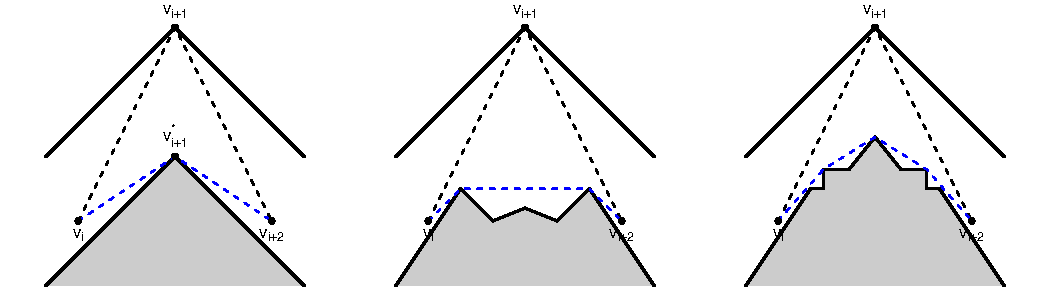
\includegraphics[width=6in]{app-WAD/figs/alterstep-proof.pdf} \\
%\caption{three panels!}
%\label{app-WAD-alterstep-dia}
%% generated by thesis/app-WAD/figs/makealterstepdia.R
%\end{figure}
%
%
%Since the ALTER step is optimal locally that shows that all triplets are are optimal and hence the whole path is optimal. So paths are shortest paths.
%


\subsection{The computational complexity of the algorithm}





